\section{Quantifying growth, process quality and causal assistance}
\label{sec:metrology}

A recursive research architecture is not supported by the observation that its repository grows or that its underlying language model eventually succeeds. A system can accumulate duplicated or irrelevant memory, spend more compute, and still attribute the model's unaided ability to the framework. We therefore treat metrology as part of the method rather than as post hoc visualization. The measurement contract is implemented prospectively in \texttt{docs/RAKL\_METROLOGY.md} and the read-only \texttt{src/rakl/v3\_metrology.py} surface on the Paper 5 challenger branch. These measurements grant no scientific or promotion authority.

\subsection{Seven-axis retained-growth vector}

The state-growth coordinates reuse the v3 saturation axes. For research cycle $t$ we define
\[
 g_t=(\Delta K_t,\Delta O_t,\Delta E_t,\Delta B_t,\Delta R_t,\Delta P_t,\Delta M_t),
\]
where the components denote retained novelty in knowledge, operators, experience patterns, obstructions, relations, successful paths and meta-methods, respectively. The qualifier \emph{retained} is essential. Raw files, commits, nodes or generated lessons are inventory, not evidence of learning. The v3 \texttt{NoveltyRound} contract records retained semantic novelty and separates it from repeated route searches or paper count.

Alongside $g_t$, each frozen state reports node counts by substrate kind, edge counts by typed relation, episode outcomes, lesson and tool authority distributions, failure-diagnosis status, evolution-variant status and unresolved cross-view links. For states $S_t$ and $S_{t+1}$, \texttt{compare\_state\_metrics} produces a content-independent growth delta. We do not collapse these quantities into a single ``lattice size'' score.

Several ratios diagnose whether growth is useful rather than merely large. We preregister lineage coverage as the fraction of derived canonical objects with valid source ancestry, unresolved-link rate in the common substrate, supersession-preservation rate, and a semantic novelty-retention ratio that compares retained additions with raw proposals once the necessary proposal identity stream is available. High raw growth with low lineage coverage or high orphan rate is a negative result, not progress.

\subsection{Experience conversion and failure learning}

The fast v3 loop stores immutable \TaskEpisode{} records; the slow loop may propose lessons, diagnoses, tools and strategy motifs. We measure the conversion funnel rather than assuming that every stored episode is useful:
\rakldisp{
\text{episodes}
\rightarrow
\text{supported diagnoses or lessons}
\rightarrow
\text{reusable tools or motifs}
\rightarrow
\text{validated fresh reuse}.
}

Reported quantities include episode outcome rates and costs, lesson proposal and validation yields, tool reuse success and failure rates, failure-diagnosis maturation, time from observation to supported diagnosis, obstruction-resolution rate, and the repeated-failure rate
\[
R_F=
\frac{\#\{\text{failures with a previously observed structural signature}\}}
     {\#\{\text{failures}\}}.
\]
A useful experience system should reduce $R_F$ on fresh tasks without increasing false transfer. Neither a high lesson yield nor a low lesson yield is intrinsically desirable. Excessive abstraction can be as harmful as failure to learn.

Table~\ref{tab:method-metrics} lists the subset of these quantities an implementer can instrument on their own long-running agent \emph{today}, independent of the (unrun) causal-attribution study. They are process-health measurements, reported as a profile, not a single ``method score''.

\begin{table}[t]
\footnotesize
\begin{tabular}{@{}p{0.27\textwidth} p{0.40\textwidth} p{0.27\textwidth}@{}}
\hline
\textbf{Metric} & \textbf{Definition} & \textbf{What it indicates} \\
\hline
Repeated-failure rate $R_F$ & failures whose structural signature was seen before, over all failures & whether the system actually learns from its own failures; target decreasing \\
Lineage coverage & derived canonical objects with valid source ancestry, over all derived objects & whether growth is grounded rather than orphaned \\
Unresolved-link / orphan rate & dangling references in the common substrate, over all links & silent decay of the knowledge base \\
Supersession-preservation rate & superseded records retained in history, over all supersessions & whether negative/old history is preserved, not overwritten \\
Invalid-promotion rate & promotions lacking a valid governed certificate, over all promotions & whether proposal/authority separation holds; target $0$ \\
\hline
\end{tabular}
\caption{Method-health metrics an implementer can instrument on a long-running agent without the causal-attribution experiment. Reported as a profile; each measures process discipline, not task accuracy.}
\label{tab:method-metrics}
\end{table}

\subsection{Process telemetry for the full method surface}

\RAKL{} already declares canonical process surfaces in \texttt{method\_specs.py}. Paper 5 requires consequential invocations to be measurable. A proposal-only \texttt{ProcessTelemetry} record binds the method surface, input and output state identities, active task and fibre, outcome, registered cost, residual transformation, retrieved/selected/rejected object identities, verification artifacts and the retained novelty vector. The common aggregate for process $p$ reports
\rakldisp{
N_p,\quad
P_p(\mathrm{success}),\quad
P_p(\mathrm{blocked}),\quad
P_p(\CANNOTCHECK),\quad
\overline C_p,\quad
\overline{\Delta |B|}_p,
}
plus axis-specific retained novelty and object-selection counts. Here $B$ denotes the registered residual set; raw residual-count contraction is descriptive because replacing one vague blocker by several precise obligations can represent epistemic progress despite increasing $|B|$.

The process-specific dashboard covers decomposition, routing, search-query generation, source qualification, claim extraction, ontology normalization, context translation, equivalence/structural transfer, contextual gluing, contradiction diagnosis, gap discovery, discriminator selection, synthesis, memory, review, benchmarking, authority promotion, saturation stopping, context compilation, capability shaping, software execution, research-portfolio allocation, objective evolution and generator transport. The complete definitions are frozen in the metrology contract. Representative quantities include atom reopen rate and late interface discovery for decomposition; saturated-route retry rate for routing; retrieval precision and recall in a bound universe for memory; hostile-near-miss rejection and false-transfer rate for transfer; local-success/global-failure rate for gluing; pre-promotion defect capture for review; exact-subject replay for software execution; and invalid promotion rate, whose target is zero.

\subsection{Residual contraction as a common progress coordinate}

Open research often lacks a scalar objective before the target theorem or artifact exists. We therefore record progress through typed residual transformations. Let $B_t$ be the canonical active blocker set for an atom. A simple contraction
\[
C_t=|B_t|-|B_{t+1}|
\]
is reported only when blocker identity is stable. The more informative representation records blockers resolved, newly exposed, unchanged and reopened. This prevents the framework from manufacturing ``progress'' by renaming an obstruction or hiding a root-like obligation inside a new representation.

\subsection{Four-arm causal-attribution benchmark}

The key empirical question is whether \RAKL{} contributes anything beyond the base model. We therefore extend the earlier reset-versus-learning design with a separate four-arm attribution benchmark (Figure~\ref{fig:four-arm}). The same frozen task packet, model revision and registered resource ceiling are used in every arm:

\begin{figure}[t]
\centering
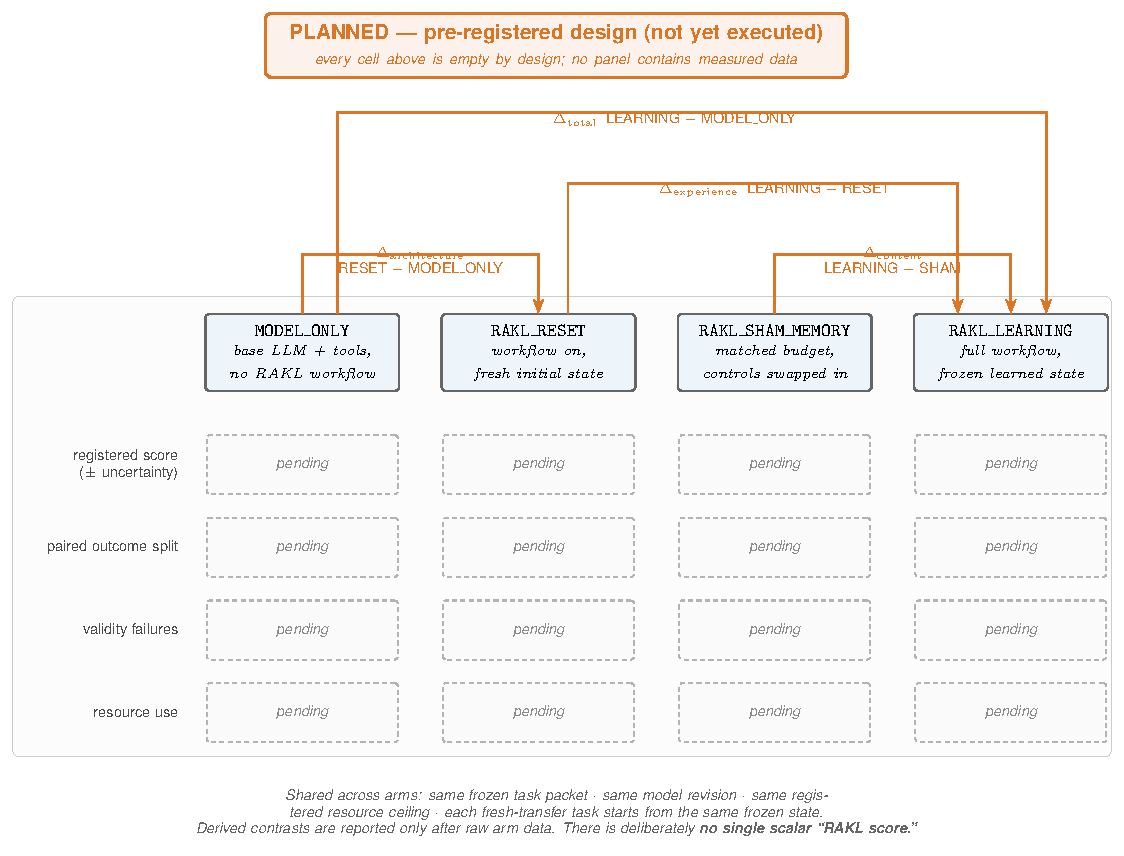
\includegraphics[width=\textwidth]{figures/four_arm_design.pdf}
\caption{The preregistered four-arm causal-attribution design (\emph{planned; not yet executed}). The arms \texttt{MODEL\_ONLY}, \texttt{RAKL\_RESET} (static architecture, fresh state), \texttt{RAKL\_SHAM\_MEMORY} (budget-matched irrelevant memory) and \texttt{RAKL\_LEARNING} isolate four separate lift contrasts: architecture ($\text{RESET}-\text{MODEL\_ONLY}$), content ($\text{LEARNING}-\text{SHAM}$), experience ($\text{LEARNING}-\text{RESET}$) and total ($\text{LEARNING}-\text{MODEL\_ONLY}$). Result cells are empty by design: this is a registered design, not a result, and there is deliberately no single scalar ``RAKL score.''}
\label{fig:four-arm}
\end{figure}

\begin{description}[leftmargin=3.2cm,style=nextline]
\item[\texttt{MODEL\_ONLY}] The same base LLM and permitted external tools operate without the \RAKL{} workflow or persistent \RAKL{} state.
\item[\texttt{RAKL\_RESET}] The \RAKL{} workflow is active, but every evaluation task starts from the same initial framework state. This estimates the static architecture effect.
\item[\texttt{RAKL\_SHAM\_MEMORY}] The workflow and memory/context budget are matched, but relevant learned memory is replaced with registered irrelevant or structurally incompatible controls. This tests whether gains arise from experience content rather than merely extra context or preprocessing.
\item[\texttt{RAKL\_LEARNING}] The full workflow uses the learned state produced by the development sequence. Every fresh-transfer task starts independently from the same frozen learned state.
\end{description}

For registered metric $m$ we report separate lift vectors
\rakldisp{
\Delta_{\mathrm{architecture}}(m)
=m(\texttt{RAKL\_RESET})-m(\texttt{MODEL\_ONLY}),
}
\rakldisp{
\Delta_{\mathrm{experience}}(m)
=m(\texttt{RAKL\_LEARNING})-m(\texttt{RAKL\_RESET}),
}
\rakldisp{
\Delta_{\mathrm{content}}(m)
=m(\texttt{RAKL\_LEARNING})-m(\texttt{RAKL\_SHAM\_MEMORY}),
}
and
\rakldisp{
\Delta_{\mathrm{total}}(m)
=m(\texttt{RAKL\_LEARNING})-m(\texttt{MODEL\_ONLY}).
}
There is deliberately no scalar ``RAKL score''.

For binary task success, each matched pair is also assigned to \texttt{BOTH\_SUCCESS}, \texttt{RAKL\_ONLY\_SUCCESS}, \texttt{BASELINE\_ONLY\_SUCCESS} or \texttt{BOTH\_FAIL}. The asymmetric counts are scientifically important. A \texttt{RAKL\_ONLY\_SUCCESS} is direct scoped evidence of assistance; a \texttt{BASELINE\_ONLY\_SUCCESS} is direct evidence that the framework interfered and must be reported with equal prominence.

\subsection{Efficiency and epistemic-safety lift}

Framework contribution is not limited to final success. When both arms solve a task we compare model tokens, preprocessing tokens, retrieval calls, tool calls, wall time, candidates attempted, failed route families and time to the first decisive falsifier. A framework that spends substantially more resources for the same result is not credited as a capability gain unless the claim is explicitly about a quantified quality or safety tradeoff.

For open research, epistemic-safety effects may appear earlier than root solutions. We therefore measure unsupported scope escalation, false theorem/candidate promotion, invalid structural transfer, surrogate-to-root coordinate errors, false global gluing, chronology violations and source-scope errors. A framework that lowers false progress while holding solution rate fixed may still be scientifically useful, but that claim is kept separate from capability improvement.

\subsection{Decision-level contribution witnesses and component ablation}

Population-level matched trials establish the main attribution. To understand mechanism, a consequential intervention may emit a proposal-only contribution witness recording what \RAKL{} consulted, how route ranking changed and what action was selected. Examples include failure memory demoting a repeated route, a retrieved tool promoting a cross-domain method, a root-coordinate preservation gate blocking a seductive surrogate, or a gluing check exposing a missing interface.

Such a witness is not causal proof. Where feasible, we preregister component ablations or leave-one-memory-out replay. Candidate ablations include removing failure memory, success-tool memory, experience-conditioned routing, problem-fibre compilation, gluing checks, saturation/invention gates, or a specific high-impact lesson. Repeated seeds or sampling configurations are required before interpreting stochastic replay differences as stable effects.

\subsection{Statistical units, dependence and uncertainty}

Tokens and tool calls are not independent observations. The primary unit is the task for matched outcome comparisons, the episode for process/failure measurements, the problem family or domain for transfer generalization, and the framework version for evolution claims. Development episodes are temporally dependent by design because the state changes. Fresh-transfer tasks must all begin from the same frozen learned state so that transfer task $T_1$ cannot train $T_2$.

We use paired analyses whenever the same task can be evaluated under multiple arms. Binary success is reported through paired contingency counts and an appropriate paired interval/test. Continuous scores and resource quantities are analysed as paired differences with bootstrap, permutation or model-based uncertainty appropriate to the frozen sampling design. If sufficient task families accumulate, hierarchical analyses will separate within-family from cross-family effects. Primary and secondary metrics, material-effect thresholds, multiplicity policy, resource ceilings, stopping rules and assurance exposure budgets are frozen before evaluated results.

\subsection{Goodhart resistance and non-compensatory invariants}

Once a metric influences upgrades it becomes a target. We therefore prohibit one-number promotion. Benchmark and evaluator hashes, thresholds and hard authority invariants are protected from the challenger they judge. Raw storage growth never counts as improvement, hostile near-misses expose over-transfer, and a gain in success or efficiency cannot compensate for an authority, history, evaluator-integrity or fresh-transfer leakage failure. If an upgrade legitimately changes a metric or evaluator definition, that evaluator migration is treated as a separately governed parent change rather than being allowed to redefine the ruler inside the challenger.

\subsection{What would demonstrate that RAKL is doing real work?}

We preregister a minimum evidentiary chain for the statement that the framework learned or assisted:
\rakldisp{
\boxed{
\text{retained semantic growth}
+\text{traceable downstream reuse/decision effect}
+\text{matched baseline lift}
+\text{fresh transfer when generalization is claimed}
+\text{no compensating validity regression}
}
}
Repository size, issue count, prose volume, proposed lesson count, or an agent's self-report that \RAKL{} was helpful do not satisfy this chain. The strongest version-level claim additionally requires protected fresh assurance and governed promotion under the upgrade protocol in Section~\ref{sec:upgrade}.